% ---------------------------------------------------------------------- %

\documentclass[letterpaper,10pt]{article}



\pagestyle{empty}

\usepackage[table]{xcolor}
\usepackage{color, colortbl}
\usepackage{tabularx}
\usepackage{amssymb}
\usepackage{enumerate}

\definecolor{LightGray}{gray}{0.9}

\usepackage{amsmath}
\usepackage{amscd}
\usepackage{url}

\usepackage{graphicx}


\title{Installing AIMBAT}
\author{Seismo Group}
\date{\today}

\begin{document}
\maketitle


% ************************************************************* %
%                                                               %
%                       INSTALLING SOD                          %
%                                                               %
% ************************************************************* %

You can get SOD from here: \url{http://www.seis.sc.edu/sod/index.html}.
Once you have gotten the folder for SOD, put it somewhere where you won't touch it too much. What I did was put the SOD folder in my home directory, though other places are acceptable as well, as long as its not too easy to delete it by accident.

\begin{figure}[h!]
  \centering
  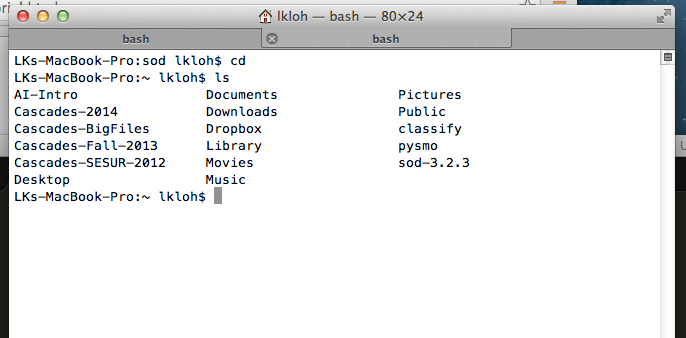
\includegraphics[width=0.5\textwidth]{images/sod_location}
  \caption{Path to sod bin}
  \label{fig:sod_location}
\end{figure}

Once you have it there, get the path to the sod folder's bin and put it in your path folder. 


\begin{figure}[h!]
  \centering
  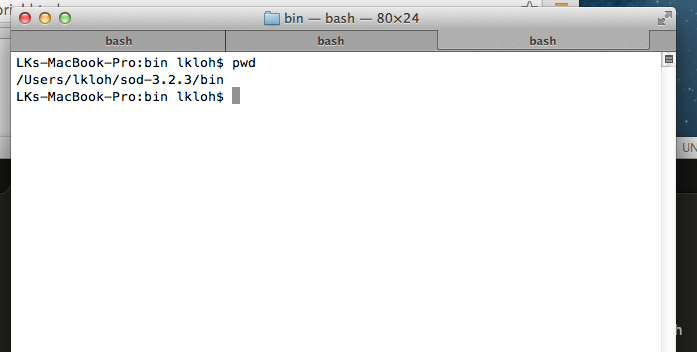
\includegraphics[width=0.5\textwidth]{images/path_to_sod_bin}
  \caption{Path to sod bin}
  \label{fig:path_to_sod_bin}
\end{figure}

Inside my home directory's bash profile (you get the by typing \verb"cd"), you put the path to \verb"sod-3.2.3/bin" by adding in either the \verb"bash" or \verb"bash_profile" or \verb"profile" files: 
 
\begin{figure}[h!]
  \centering
  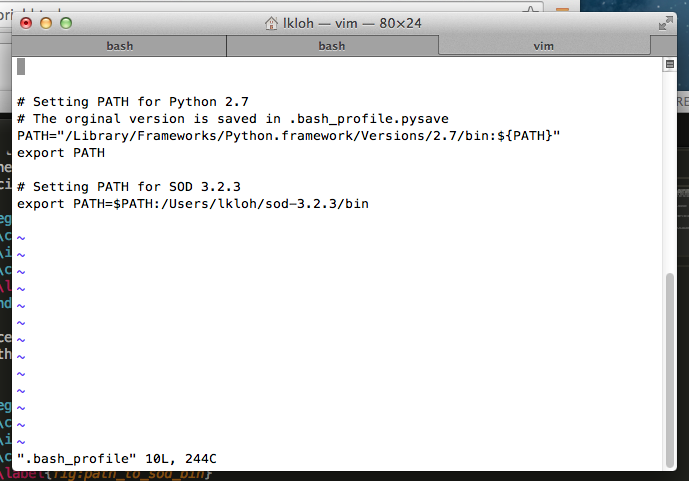
\includegraphics[width=0.5\textwidth]{images/home_bash_profile}
  \caption{bash profile}
  \label{fig:home_bash_profile}
\end{figure}

To check if SOD has been installed properly, close the terminal, restart it, and type \verb"sod". If that works, we should see something like this: 

\begin{figure}[h!]
  \centering
  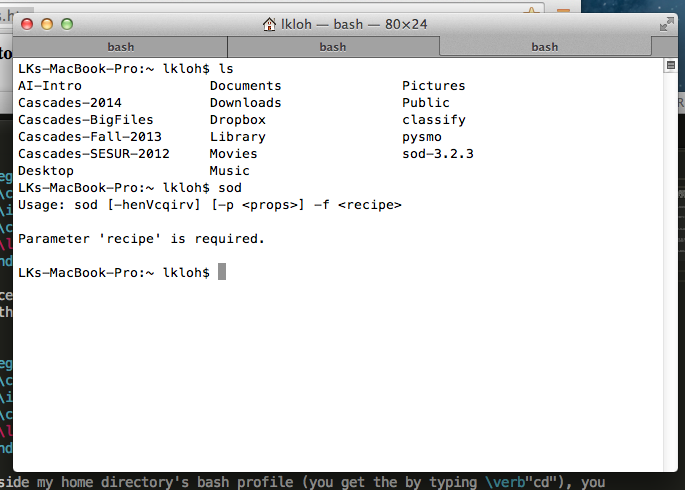
\includegraphics[width=0.5\textwidth]{images/sod_installed_query}
  \caption{Is SOD installed?}
  \label{fig:sod_installed_query}
\end{figure}




% ------------------------------------------------------------------------- %


\end{document}

% --------------------------------- END --------------------------------- %
